\subsubsection{\theoryC{Sensitivity to heavy Higgs bosons in models with vectorlike quarks and leptons at the HL- and HE-LHC}}
\contributors{Radovan Dermisek, Enrico Lunghi, Seodong Shin}\rt{There are comments to address. We can maybe remove the figure with diagrams.}
%{\bf Author(s): Radovan Dermisek, Enrico Lunghi, Seodong Shin}
%
%
%Radovan Dermisek: Physics Department, Indiana University, Bloomington, IN 47405, USA \\
%dermisek@indiana.edu \\
%Enrico Lunghi: Physics Department, Indiana University, Bloomington, IN 47405, USA \\
%elunghi@indiana.edu \\
%Seodong Shin: Enrico Fermi Institute, University of Chicago, Chicago, IL 60637, USA \\
%Department of Physics and IPAP, Yonsei University, Seoul 03722, Korea \\
%shinseod@indiana.edu, seodongshin@yonsei.ac.kr
%

%\subsubsection{Introduction}
%\paragraph*{Introduction}

Among the simplest extensions of the standard model (SM) are models with extended Higgs sector and models with additional vectorlike matter. 
Although many search strategies for individual new particles were designed, there are large regions of the parameter space that HL- or HE-LHC will not be sensitive to as a result of either small production rates or large SM backgrounds.  However, combined signatures of both extra sectors can lead to many new opportunities to search for heavy Higgs bosons and vectorlike matter simultaneously~\cite{Dermisek:2015hue}. 

For example, in a type-II two Higgs doublet model, the production cross section of the 1 TeV heavy \cpeven \rt{Define command for \cpeven/odd?}  Higgs boson can be as sizable as $\sim 2$ pb (10 pb) at 13TeV (27TeV) \com energy, depending on the values of $\tan\beta$.
However, in the decoupling limit, where $H \to ZZ,\; WW$ are suppressed or not present, the dominant decay modes are $t\bar t$, $hh$, $b\bar b$ and $\tau^+\tau^-$ which suffer from large SM backgrounds or small branching fractions in some regions of $\tan \beta$. On the other hand, vectorlike leptons typically have very clean signatures but their production rates are very small. Nevertheless, since vectorlike leptons can appear in decay chains of  heavy Higgs bosons, the combined signature can feature both the sizable production rate and clean final states. 

%We consider the extension of the type-II two Higgs doublet model by vectorlike pairs of quarks and leptons introduced in \citeref{Dermisek:2015oja}. 
%In the following sections we briefly outline the model, summarize possible heavy Higgs cascade decays through vectorlike quarks and leptons and discuss  the sensitivity of the HL- and HE-LHC for selected decay modes.


%\subsubsection{Model Framework}
%\paragraph*{Model Framework}

We consider a type-II two Higgs doublet model augmented by vectorlike pairs of new quarks (SU(2) doublets $Q_{L,R}$ and SU(2) singlets $U_{L,R}$ and $D_{L,R}$)
and vectorlike pairs of new leptons (SU(2) doublets $L_{L,R}$,  SU(2) singlets $E_{L,R}$ and  SM singlets $N_{L,R}$)~ \cite{Dermisek:2015oja}. The  $Q_{L}$, $U_{R}$,  $D_{R}$, $L_L$ and $E_R$ have the same  hypercharges as quarks and leptons in the SM, as summarized in \tabb{table:fieldcontents}.
We  further assume that the new leptons mix only with one family of SM leptons in order to simply avoid strong constraints from the experiments searching for lepton flavor violation and we consider the mixing with the second family as an example~\cite{Kannike:2011ng,Dermisek:2013gta,Falkowski:2013jya,Falkowski:2014ffa,Dermisek:2014cia,Dermisek:2014qca,Dermisek:2015vra,Dermisek:2015oja,Dermisek:2015hue,Dermisek:2016via} (the discovery potential in the case of mixing with the first family would be comparable~\cite{Dermisek:2014qca} and in the case of mixing with the third family it would be significantly weaker~\cite{Dermisek:2014qca,Kumar:2015tna}). This can be achieved by requiring that the individual lepton number is an approximate symmetry (violated only by light neutrino masses). Similarly,  we assume that the new quarks mix only with the third family of SM quarks. We consider the most general renormalizable Lagrangian consistent with these assumptions.

%%%-------------------------
\begin{table}[htp]
    \caption{Quantum numbers of standard model leptons and quarks ($\ell^i_L$, $e^i_R$, $q^i_L, u^i_R, d^i_R$ for $i=1,2,3$), extra vectorlike leptons and quarks and the two Higgs doublets. The electric charge is given by $Q = T_3 +Y$, where $T_3$ is the weak isospin, which is +1/2 for the first component of a doublet and -1/2 for the second component. }
\begin{center}
\resizebox{\columnwidth}{!}{
\begin{tabular}{c c c c c c c c c c c c c c}
\hline
\hline
 & ~~$\ell^i_L$ & ~~$e^i_R$ & ~~$q^i_L$ & ~~$u^i_R$ & ~~$d^i_R$ & ~~$L_{L,R}$ & ~~$E_{L,R}$ & ~~$N_{L,R}$ & ~~$Q_{L,R}$ & ~~$T_{L,R}$ & ~~$B_{L,R}$ & ~~$H_d$ & ~~ $H_u$\\
\hline
SU(2)$_{\rm L}$ & ~~\bf 2 & ~~\bf 1 & ~~\bf 2 & ~~\bf 1 & ~~\bf 1 & ~~\bf 2 & ~~\bf 1 & ~~\bf 1 & ~~\bf 2 & ~~\bf 1 & ~~\bf 1 & ~~\bf 2 & ~~\bf 2 \\
U(1)$_{\rm Y}$ & ~~$-\frac12$ & ~~-1 & ~~$\frac16$ & ~~$\frac23$ & ~~-$\frac13$ & ~~$-\frac12$ & ~~-1 & ~~0  & ~~$\frac16$ & ~~$\frac23$ & ~~-$\frac13$ & ~~$\frac12$ & ~~-$\frac12$ \\
Z$_2$ & ~~+ & ~~- & ~~+ & ~~+ & ~~-- & ~~+ & ~~- & ~~+ & ~~+ & ~~+ & ~~-- & ~~-- & ~~+ \\
\hline
\hline
\end{tabular}}
\end{center}
\label{table:fieldcontents}
\end{table}
%%%-----------------------

Details of the lepton sector of the model were worked out in \citeref{Dermisek:2015oja}.
After spontaneous symmetry breaking, $\left< H_u^0 \right> = v_u$ and $\left< H_d^0 \right> = v_d$ with $\sqrt{v_u^2 + v_d^2} = v = 174$ GeV (we also define $\tan \beta \equiv v_u / v_d$), the model can be summarized by mass matrices in the charged lepton sector, with left-handed fields $( \bar \mu_{L}, \bar L^-_L, \bar E_L )$ on the left and right-handed fields $( \mu_{R} , L^-_R, 
 E_R)^T$ on the right~\cite{Dermisek:2013gta},
\begin{eqnarray}
M_e \;  
%
&=& 
%
\begin{pmatrix}
 y_\mu v_d & 0 &  \lambda_E v_d\\
  \lambda_L v_d & M_L &  \lambda v_d\\
 0 & \bar \lambda v_d & M_E 
\end{pmatrix},
\end{eqnarray}
%
and in the neutral lepton sector, with left-handed fields $( \bar \nu_\mu , \bar{L}_L^0 , \bar N_L)$ on the left and right-handed fields $( \nu_R = 0 ,
L_R^0 ,
N_R)^T$ on the right~\cite{Dermisek:2015oja},
%
\begin{eqnarray}
M_\nu  &=& 
\left( 
\begin{array}{ccc}
0 & 0 & \kappa_N v_u \\
0 & M_L & \kappa v_u \\
0 & \bar \kappa v_u & M_N \\
\end{array}
\right)~.
\label{eq:mm}
\end{eqnarray}
%
The superscripts on vectorlike fields represent the charged and the neutral components (we  inserted $\nu_R = 0$ for the  right-handed neutrino which is absent in our framework in order to keep  the mass matrix $3\times3$ in complete analogy with the charged sector).  The usual SM Yukawa coupling of the muon is denoted by $y_\mu$, the Yukawa couplings to $H_d$ are denoted by various $\lambda$s, the Yukawa couplings to $H_u$ are denoted by various $\kappa$s, and finally the explicit mass terms for vectorlike  leptons are given by $M_{L,E,N}$. Note that explicit mass terms between SM and vectorlike fields (i.e. $\bar \mu_L L_R$ and $\bar E_L \mu_R$) can be rotated away. These mass matrices can be diagonalized by bi-unitary transformations and we label the two new charged and neutral mass eigenstates by $e_4, \, e_5$ and $\nu_4, \, \nu_5$ respectively:
%
\begin{eqnarray}
U_L^\dagger M_e U_R &=& {\rm diag}
\left(
 m_\mu,  m_{e_4} ,  m_{e_5}
\right), \\
V_L^\dagger M_\nu V_R &= &  {\rm diag} 
\left(0, m_{\nu_4} , m_{\nu_5}
\right).
\label{eq:unitary}
\end{eqnarray}
%

Since SU(2) singlets mix with SU(2) doublets \rt{We have to uniform notation for groups, such as SU(2), U(1) etc.}, the couplings of all involved particles to the $Z$, $W$ and Higgs bosons are in general modified. The flavor conserving couplings receive corrections and flavor changing couplings between the muon (or muon neutrino)  and heavy leptons are generated. The relevant formulas for these couplings in terms of diagonalization matrices defined above can be found in \citerefs{Dermisek:2015oja, Dermisek:2013gta}. In the limit of small mixing, approximate analytic expressions  for diagonalization matrices can be obtained which are often useful for the understanding of numerical results. These are also given in \citerefs{Dermisek:2015oja, Dermisek:2013gta}.

Details of the quark sector of the model can be found in \citeref{future}.
The mass matrix in the up and down quark sectors closely follow those for the neutrino and the charged leptons above. 


%\subsubsection{Heavy Higgs cascade decays through vectorlike leptons}
%\paragraph*{Heavy Higgs cascade decays through vectorlike leptons}
%
%
%\paragraph*{Signatures and search strategies}

The generated flavor changing couplings between heavy and light leptons lead to new decay modes of heavy \cpeven (or \cpodd) Higgs boson: $H \to \nu_4 \nu_\mu$ and $H \to e_4 \mu$, where $e_4$ and $\nu_4$ are the  lightest new charged and neutral leptons. The branching ratios for these decay modes can be very large when the mass of  the heavy Higgs boson is below the $t \bar t$ threshold and the light Higgs boson ($h$) is SM-like so that $H \to ZZ,\; WW$ are suppressed or not present. In this case, flavor changing decays $H \to \nu_4 \nu_\mu$ or $H \to e_4 \mu$ compete only with $H\to b \bar b$,  and for sufficiently heavy $H$, also with $H \to hh$. 
Subsequent decay modes of $e_4$ and $\nu_4$, $e_4 \to W  \nu_\mu$, $e_4 \to Z \mu$,  $e_4 \to h \mu$ and $\nu_4 \to W \mu$, $\nu_4 \to Z \nu_\mu$, $\nu_4 \to h \nu_\mu$ lead to the following 6 decay chains of the heavy Higgs boson:
%
\begin{align}
H &\; \to \; \nu_4 \nu_\mu \; \to \; W\mu \nu_\mu, \; Z\nu_\mu \nu_\mu,\; h \nu_\mu \nu_\mu~, \label{eq:Hn4} \\  
H &\; \to \; e_4 \mu \; \to \; W\nu_\mu \mu, \; Z\mu\mu,\; h \mu\mu~, \label{eq:He4}
\end{align}
%
 which are also depicted in \fig{fig:topologies}. In addition, $H$ could also decay into pairs of vectorlike leptons. This is however  limited to smaller ranges for masses in which these decays are kinematically open. Moreover, the final states are the same as in pair production of vectorlike leptons. We will not consider these possibilities here. Finally, although we  focus on the second family of SM leptons in final states, the modification for a different family of leptons or quarks is straightforward.


In \citeref{Dermisek:2015hue}, it was found that in a large range of the parameter space branching ratios for the decay modes \eqref{eq:Hn4} and \eqref{eq:He4} can be sizable  or even dominant while satisfying constraints from searches for heavy Higgs bosons,  pair production of  vectorlike leptons~\cite{Dermisek:2014qca} obtained from searches for anomalous production of multilepton events, and  constraints from precision EW observables~\cite{Patrignani:2016xqp}.
Since the Higgs production cross section can be very large, for example the cross section for a 200 GeV Higgs boson at 13 TeV (27 TeV)  LHC for $\tan \beta =1$ is 18pb (67pb)~\cite{Heinemeyer:2013tqa,Harlander:2012pb,Harlander:2016hcx}, the final states above can be produced in large numbers. Thus searching for these processes could  lead to the simultaneous discovery of a new Higgs boson and a new lepton. Some of the decay modes in \fig{fig:topologies} also allow for full reconstruction of the masses of both new particles in the decay chain.
%
\begin{figure}
\begin{center}
%
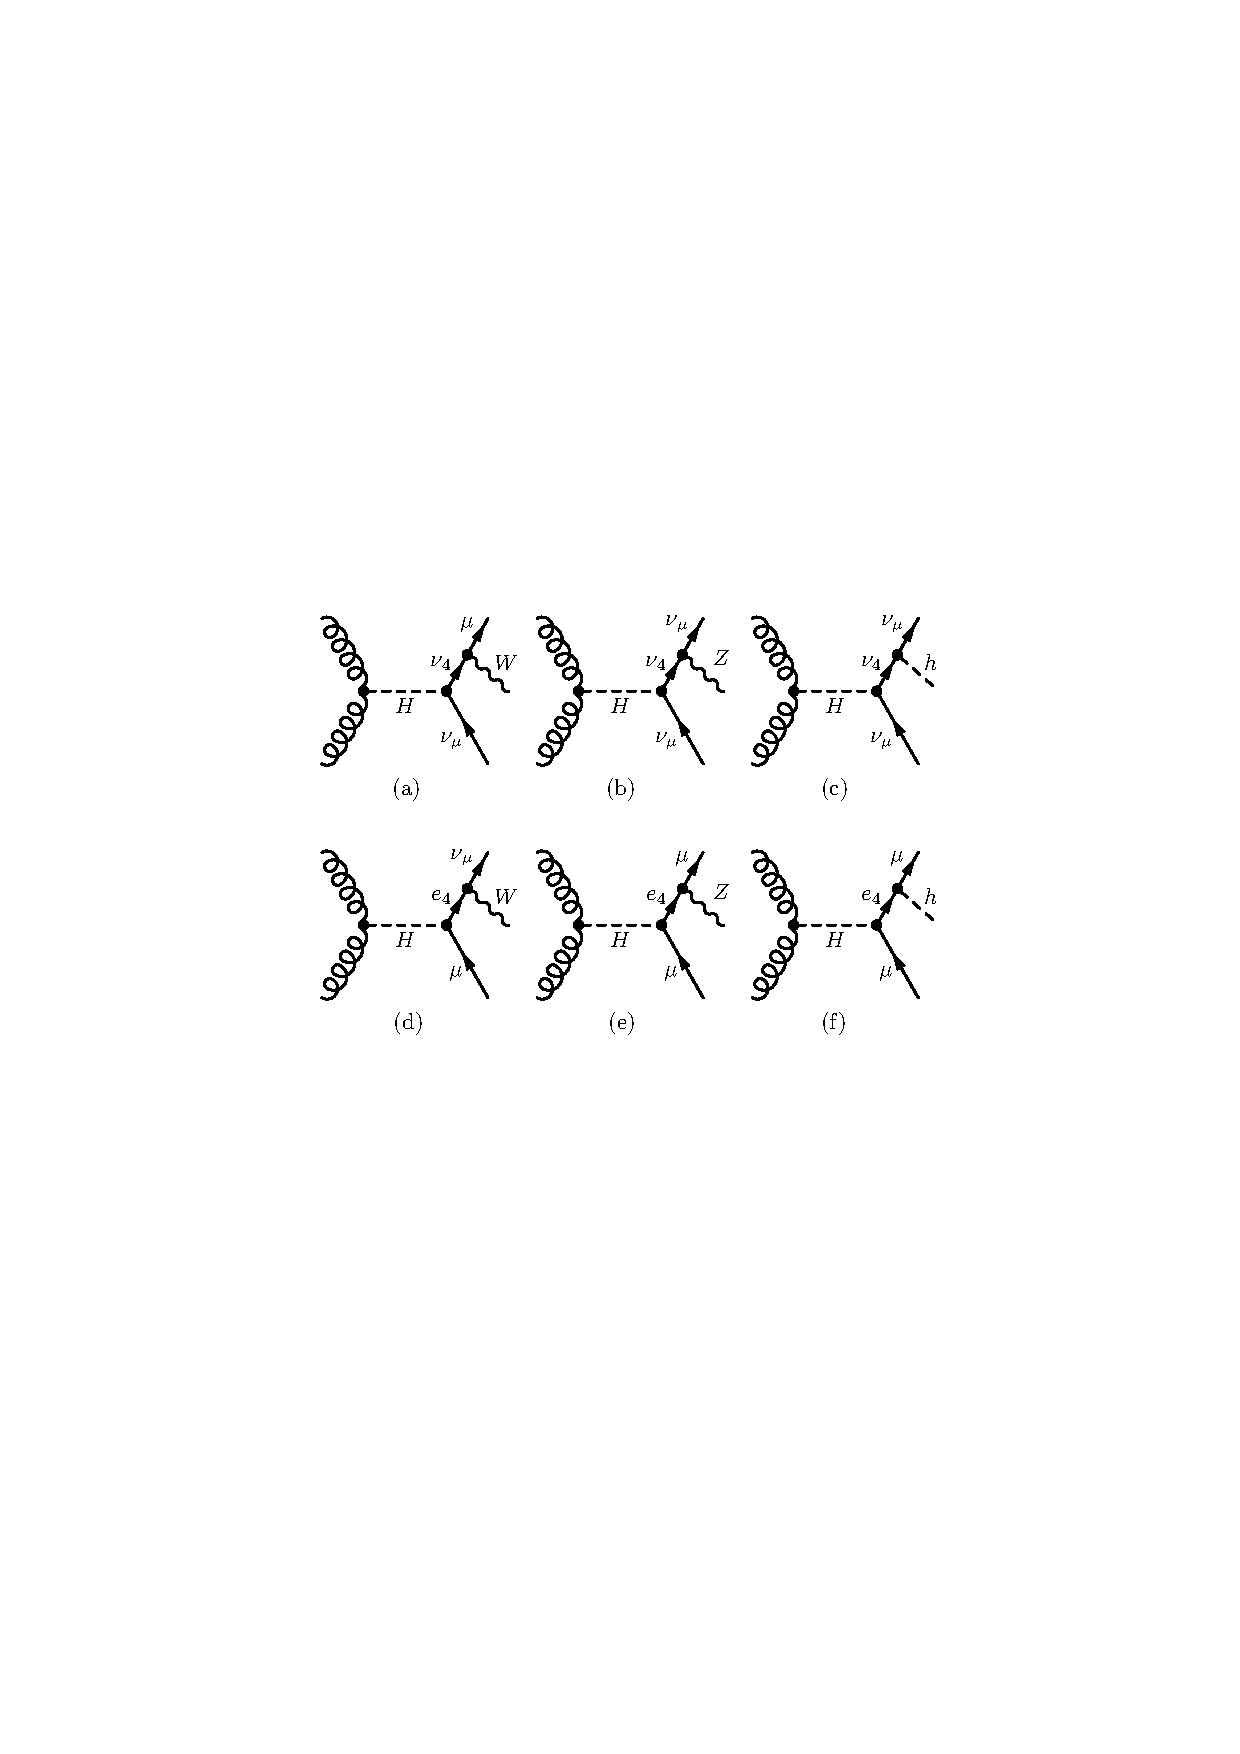
\includegraphics[width=0.5\linewidth]{\main/section7OtherSignatures/img/fig1.pdf}
%
\caption{Heavy Higgs boson cascade decays through vectorlike leptons.
\label{fig:topologies}
}
\end{center}
\end{figure}
%


The final states of the processes \eqref{eq:Hn4} and \eqref{eq:He4} are the same as final states of $pp \to WW, ZZ, Zh$ production or $H \to WW, ZZ$ decays with one of the gauge bosons decaying into second generation of leptons.  Since searching for leptons in final states is typically advantageous,  our processes contribute to a variety of existing searches.  Even searches for processes with fairly large cross sections can be significantly affected. For example, the contribution of  $pp \to H \to \nu_4 \nu_\mu \to W \mu \nu_\mu$  to $pp \to WW$ can be close to current limits while satisfying the constraints from  $H \to WW$. This has been studied in \citeref{Dermisek:2015oja} in the two Higgs doublet model we consider here, and also in a more model independent way in \citeref{Dermisek:2015vra}. 

The discussion of the main features of each of the heavy Higgs decay modes, of existing experimental searches to which these new process contribute, and of possible new searches can be found in \citeref{Dermisek:2015hue}. 
The processes with small SM backgrounds are the best place to look for this scenario. Examples include $H \; \to \; h \nu_\mu \nu_\mu$ and $H \; \to \; h \mu\mu$ with $h\to \gamma \gamma$. 


%\paragraph*{Reach of the HL- and HE-LHC}

We now discuss the parameter regions of heavy Higgses and vectorlike leptons which can be accessed by dedicated searches for the modes we propose with current LHC (36 fb$^{-1}$), HL- and HE-LHC. Among the processes depicted in \fig{fig:topologies}, we choose $H \to e_4^\pm \mu^\mp \to h \mu^+ \mu^-$  and $H \to e_4^\pm \mu^\mp \to Z \mu^+ \mu^-$ as representative examples. These are interesting because they result in additional resonances. The first process was analyzed in \citeref{Dermisek:2016via} for $m_H \le 340$ GeV. The key selection criterium is an {\it off-$Z$} cut ($|m_{\mu^+ \mu^-} - M_Z| > 15\,{\rm GeV}$) which exploits the fact that the invariant mass of the two muons in the final state is distributed mostly outside of the $Z$ boson resonance region. This cut removes to a large extent background events from $Z$ + (heavy flavored) jets with $Z \to \mu^+ \mu^-$ and raises enormously the signal significance~\cite{Dermisek:2016via}. In order to maximize the signal cross section, we focus on $h \to b \bar{b}$ (which we studied in detail in \citeref{Dermisek:2016via}) and $Z \to b \bar{b}$.

To obtain the expected sensitivities, we estimate the number of background events for the HL-LHC by rescaling the results of \citeref{Dermisek:2016via} (which are based on the search for a heavy resonance decaying to $hZ$ at ATLAS~\cite{TheATLAScollaboration:2016loc}) by the ratio of luminosities. We further estimate that the backgrounds at the HE-LHC increase by a factor $3.6 \times 5$ with respect to those at the HL-LHC, where 3.6 is the ratio of the background cross sections calculated with MadGraph5 and 5 comes from the ratio of integrated luminosities (15 ab$^{-1}$ / 3 ab$^{-1}$).

We take a flat signal acceptance of about 30\% for $m_H \le 800\,{\rm GeV}$ based on the analysis presented in \citeref{Dermisek:2016via} for $m_H = 450, 550, 650, 750$ GeV and $m_{e_4} = 250$ GeV. For $m_H \ge 800\,{\rm GeV}$ the dimuon invariant mass is much harder and concentrated above the $Z$ resonance; in this region we assume an acceptance of about 50\%. Furthermore, we consider a flat 50\% detector efficiency throughout this analysis.

These estimates of background events, signal acceptances, and detector efficiencies, allow us to calculate the corresponding experimental sensitivities using the condition:
%
\begin{align}
N_s^{95} \le \sigma_H \cdot {\rm BR}(H \to e_4 \mu) \cdot {\rm BR} (e_4 \to h \mu,\, Z \mu) \cdot A \cdot \epsilon \cdot \mathcal L\,,
\end{align}
%
where $\sigma_H$ is the $pp\to H$ production cross section, $A$ is the signal acceptance, $\epsilon$ is the experimental efficiency, and $\mathcal L$ is the integrated luminosity. $N_s^{95}$ is the 95\%~\cl upper limit on the expected number of events calculated from the background estimations described above using a modified frequentist construction (CLs)~\cite{bib-cls} based on a Poisson distribution. 

%--
\begin{figure}
\centering
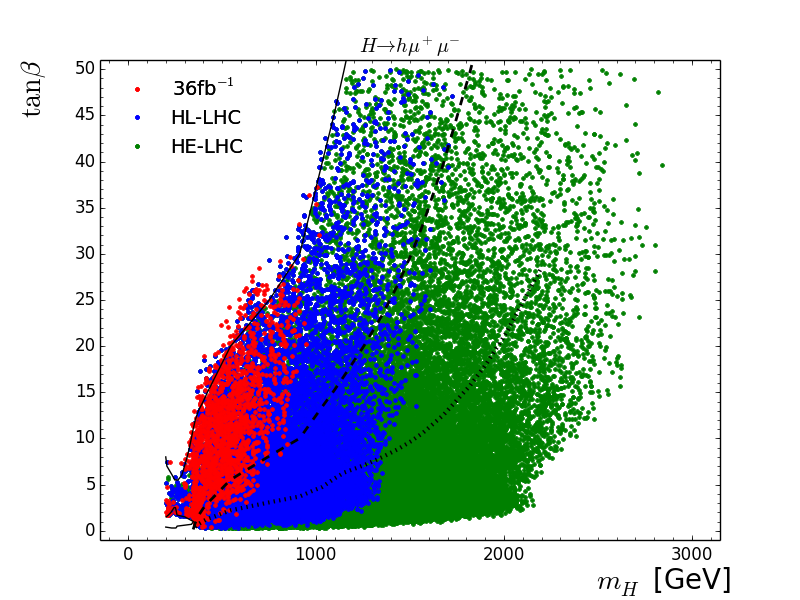
\includegraphics[width=0.49\linewidth]{\main/section7OtherSignatures/img/fig-HEHL-mH-tanbe-hmumu.png}
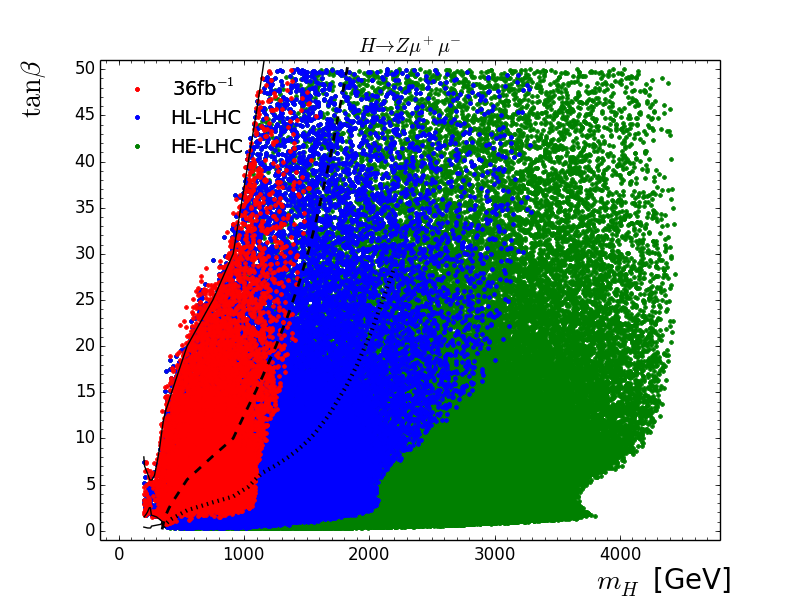
\includegraphics[width=0.49\linewidth]
{\main/section7OtherSignatures/img/fig-HEHL-mH-tanbe-Zmumu.png}
\caption{
Experimental sensitivities for $H \to e_4^\pm \mu^\mp \to h \mu^+ \mu^-$ (left) $H \to e_4^\pm \mu^\mp \to Z \mu^+ \mu^-$ (right). Red, blue and green points are the regions of the $[m_H,\tan\beta]$ plane which are accessible with LHC with $36$ fb$^{-1}$, at the HL-LHC, and at the HE-LHC, respectively. Black solid, dashed and dotted lines represent the corresponding reaches of $H\to \tau\tau$ searches.}
\label{fig:mHtanbe}
\end{figure}
%--

Among the conventional searches of neutral heavy Higgs bosons, $H \to \tau^+ \tau^-$~\cite{Aaboud:2017sjh} currently provides the strongest constraints on our model, especially for large $\tan\beta$ region; we expect that future analysis improvements may boost the impact of $H \to b \bar b$ and $H \to t \bar t$. Searches for $H \to WW$ and $H\to ZZ$ are not constraining because these decays are heavily suppressed in the alignment limit in which tree--level couplings of heavy Higgs and weak gauge bosons vanish. Nevertheless, the processes $H \to e_4 \ell (\nu_4 \nu_\ell) \to \nu_\ell \ell W$ and $H \to e_4 \ell \to \ell^+ \ell^- Z$ are indirectly constrained by searches for $H \to WW$ and $H\to ZZ$ albeit with different kinematic topologies~\cite{Dermisek:2015vra, Dermisek:2015oja, Dermisek:2015hue}. 
%We leave a more detailed analyses of the $H \to WW, ZZ$ constraints at the HL- and HE-LHC to future work. 
The decay $H \to \gamma \gamma$ currently constraints our model at small $\tan\beta \lesssim 1.5$ (at the HL-LHC values of $\tan\beta$ for which we expect constraints raises to about 3.5).  Here we focus on $H \to \tau^+ \tau^-$ as a competitive search avenue for a heavy neutral Higgs boson. 

Let us comment on the extraction of the experimental sensitivities to $H\to \tau\tau$ mentioned above. We assume that there is no change in cut acceptances and detector efficiencies for $H\to\tau\tau$ (for a given $m_H$) for the HL-LHC and the HE-LHC,\footnote{This is reasonable because the kinematics of $H$ decay products depends almost exclusively on $m_H$.} implying that $S / \sqrt{B}$ controls to a good approximation the change in sensitivity. With this assumptions, the sensitivity at the HL-LHC increases simply by the square-root of the ratio of the integrated luminosities, i.e., $\sqrt{3000./36.} = 9.13$.\rt{This is true when the statistics is large. When approaching $N_{B}=$few (that should be at the edge of the constraint) I expect the limit to scale linearly with the integ. lumi.} For the HE-LHC, we can obtain the sensitivities by further assuming that the background production cross sections ($\sigma_{\rm bkg.}$) increase by the ratio of Higgs production cross sections for $\tan\beta = 1$, i.e., $\sigma_{\rm bkg.}^{\rm 13\, TeV} / \sigma_{\rm bkg.}^{\rm 27\, TeV} = \sigma (p p \to H)^{\rm 27 TeV}_{\tan\beta = 1} / \sigma (p p \to H)^{\rm 13 TeV}_{\tan\beta = 1}$, and that the background cut acceptances remain constant.\rt{Why BG CS should increase as signal CS at $\tan\beta=1$?} Then, the sensitivity increases as follows:
%--
\begin{align}
\frac{{\rm S}^{{\rm 27\,TeV,~15\,ab}^{-1}}}{\sqrt{{\rm B}^{{\rm 27\,TeV,~15\,ab}^{-1}}}} 
&= 
\frac{{\rm S}^{{\rm 13\,TeV,~36\,fb}^{-1}}}{\sqrt{{\rm B}^{{\rm 13\,TeV,~36\,fb}^{-1}}}} \cdot \frac{\sigma(p p \to H \to \tau^+ \tau^-)^{\rm 27\,TeV}}{\sigma(p p \to H \to \tau^+ \tau^-)^{\rm 13\,TeV}} \cdot \sqrt{\frac{\sigma_{\rm bkg.}^{\rm 13\,TeV}}{\sigma_{\rm bkg.}^{\rm 27\,TeV}} \cdot \frac{\mathcal{L}^{{\rm 15\,ab}^{-1}}}{\mathcal{L}^{{\rm 36\,fb}^{-1}}}}  
\nonumber \\
& \hskip -1cm = 
\frac{{\rm S}^{{\rm 13\,TeV,~36\,fb}^{-1}}}{\sqrt{{\rm B}^{{\rm 13\,TeV,~36\,fb}^{-1}}}} \cdot \frac{\sigma(p p \to H \to \tau^+ \tau^-)^{\rm 27\,TeV}}{\sigma(p p \to H \to \tau^+ \tau^-)^{\rm 13\,TeV}} \cdot 20.4 \cdot \sqrt{\frac{\sigma (p p \to H)^{\rm 13 TeV}_{\tan\beta = 1}}{\sigma (p p \to H)^{\rm 27 TeV}_{\tan\beta = 1}}} 
\,,
\label{eq:VLFsensitivity}
\end{align}
%--
where ${\rm S}^{{\rm 27\,TeV,~15\,ab}^{-1}}$ (${\rm S}^{{\rm 13\,TeV,~36\,fb}^{-1}}$) and ${\rm B}^{{\rm 27\,TeV,~15\,ab}^{-1}}$ (${\rm B}^{{\rm 13\,TeV,~36\,fb}^{-1}}$) are the number of signal and background events for $H \to \tau^+ \tau^-$ at the HE-LHC (at the LHC with 36\,fb$^{-1}$). Note that the estimated sensitivity in \eq{eq:VLFsensitivity} does not include experimental systematic uncertainties, that would somewhat weaken the reach of $H\to \tau\tau$.

Our main results are presented in \figs{fig:mHtanbe}, \ref{fig:scancombinedbr} and \ref{fig:mHme4}, where we show the experimental sensitivities for $H \to e_4^\pm \mu^\mp \to h \mu^+ \mu^-$ (left) $H \to e_4^\pm \mu^\mp \to Z \mu^+ \mu^-$ (right) obtained from reanalysing current data with integrated luminosity 36 fb$^{-1}$ (red), our estimates for the HL-LHC (blue), and HE-LHC (green). For comparison, in \fig{fig:mHtanbe}, the reach of $H \to \tau^+ \tau^-$ searches in conventional type-II two Higgs doublet model with the current data, at the HL-LHC, and the HE-LHC are shown as black solid, dashed, and dotted lines, respectively. The scatter points satisfy constraints from electroweak precision tests, Drell-Yan pair production of vectorlike leptons~\cite{Dermisek:2014qca}, heavy Higgs searches in the $H \to \tau^+ \tau^-$~\cite{Aaboud:2017sjh} and $H \to \gamma \gamma$~\cite{Khachatryan:2016yec, Aaboud:2017yyg} channels. The range of parameters that we scan over is:
%
\begin{align}
M_{L,N} &\in [100, 5000] {\rm GeV} \; , \\
\lambda_L, \lambda_E, \lambda, \bar \lambda &\in [-1, 1] \; , \\
\kappa_N = \kappa = \bar \kappa &= 0 \; , \\
\tan\beta & \in [0.3, 50] \; .
\label{eq:scan}
\end{align}
%

From the inspections of \fig{fig:mHtanbe}, we see that searches for heavy Higgs cascade decays into vectorlike leptons considerably extend the reach beyond that of $H\to \tau^+\tau^-$. Searches for $H\to h\mu^+\mu^-$ are sensitive to $m_H$ up to 1.7 TeV (2.9 TeV) and $m_{e_4}$ up to 1 TeV (1.8 TeV) at the HL-LHC (HE-LHC). The decay mode $H\to Z\mu^+\mu^-$ is even more promising and extends the sensitivity to $m_H$ up to 3.3 TeV (4.5 TeV) and $m_{e_4}$ up to 2.2 TeV (3.5 TeV) at the HL-LHC (HE-LHC).\rt{I have shortened a bit removing the last part on vector-like quarks, since it sis not contain final results.}

%--
%\begin{align}
%\sqrt{\frac{\sigma (p p \to H)^{\rm 13 TeV}_{\tan\beta = 1}}{\sigma (p p \to H)^{\rm 27 TeV}_{\tan\beta = 1}} \cdot \frac{\mathcal{L}^{{\rm 15\,ab}^{-1}}}{\mathcal{L}^{{\rm 36\,fb}^{-1}}}} = 20.4 \cdot \sqrt{\frac{\sigma (p p \to H)^{\rm 13 TeV}_{\tan\beta = 1}}{\sigma (p p \to H)^{\rm 27 TeV}_{\tan\beta = 1}}}\,.
%\end{align}
%--
%Note that the same level of experimental sensitivities are obtained as 
%--
%\begin{align}
%\frac{{\rm S}^{{\rm 27\,TeV,~15\,ab}^{-1}}}{\sqrt{{\rm B}^{{\rm 27\,TeV,~15\,ab}^{-1}}}} &= \frac{{\rm S}^{{\rm 13\,TeV,~36\,fb}^{-1}}}{\sqrt{{\rm B}^{{\rm 13\,TeV,~36\,fb}^{-1}}}} \hspace{0.5cm} {\rm if~and~only~if} \nonumber \\
%& \sigma(p p \to H \to \tau^+ \tau^-)^{\rm 27\,TeV} = \frac{\sigma(p p \to H \to \tau^+ \tau^-)^{\rm 13\,TeV}}{20.4 \cdot \sqrt{\frac{\sigma (p p \to H)^{\rm 13 TeV}_{\tan\beta = 1}}{\sigma (p p \to H)^{\rm 27 TeV}_{\tan\beta = 1}}}}\,.
%\end{align}
%--


%--
\begin{figure}
\centering
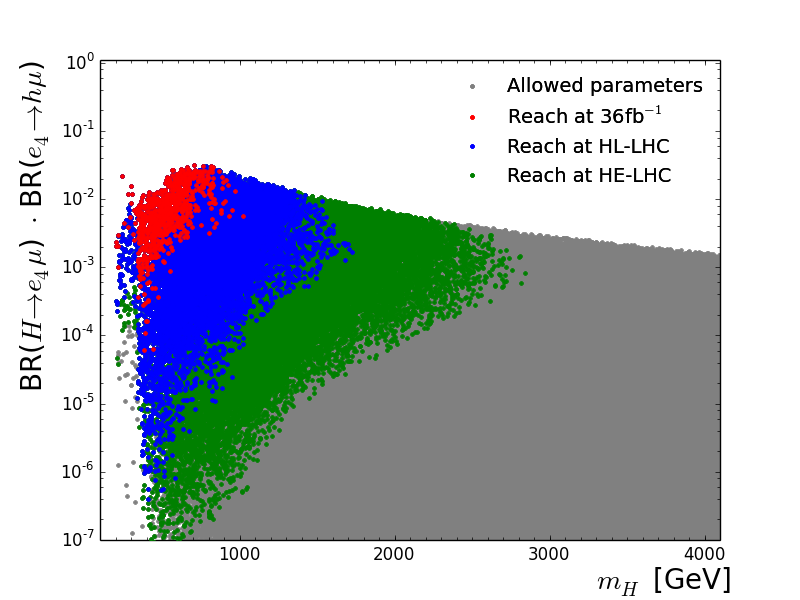
\includegraphics[width=0.49\linewidth]{\main/section7OtherSignatures/img/fig-HEHL-mH-BRHhmm.png}
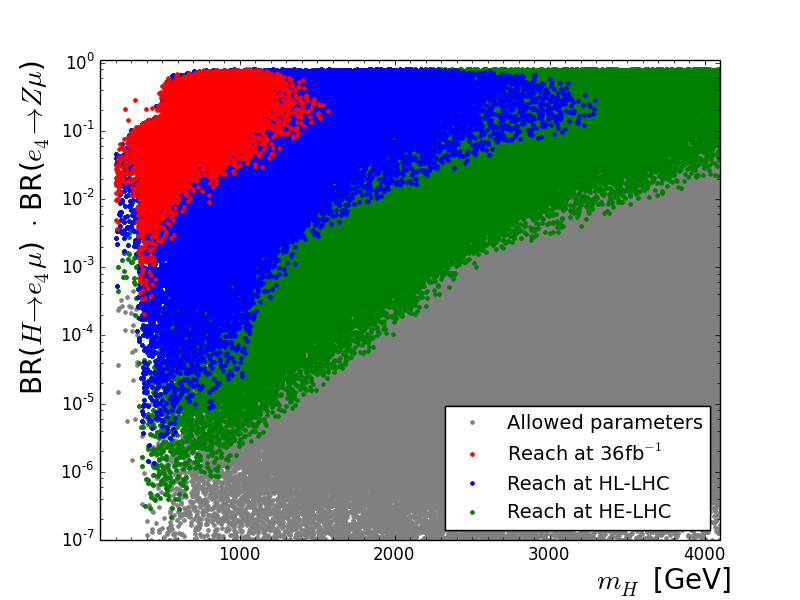
\includegraphics[width=0.49\linewidth]{\main/section7OtherSignatures/img/fig-HEHL-mH-BRHzmm.png}
\caption{
Possible values of the branching ratios ${\rm BR}(H \to e_4 \mu) \times {\rm BR}(e_4 \to h \mu)$ (left) and ${\rm BR}(H \to e_4 \mu) \times {\rm BR}(e_4 \to Z \mu)$ (right) as a function of $m_H$. Note that ${\rm BR}(H \to e_4 \mu)$ includes both $H \to e_4^+ \mu$ and $H \to e_4^- \mu^+$ decay modes. See the caption in \fig{fig:mHtanbe} for further details.
}
\label{fig:scancombinedbr}
\end{figure}
%--

%--
\begin{figure}
\centering
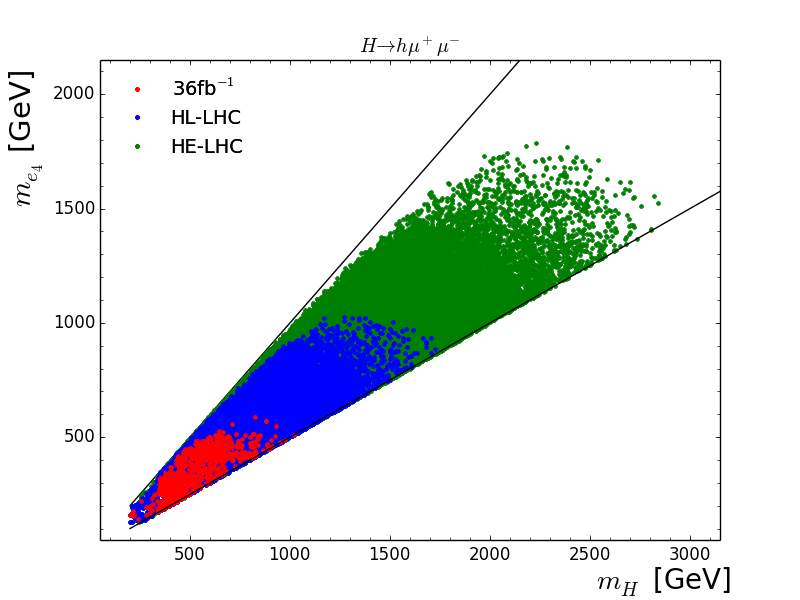
\includegraphics[width=0.49\linewidth]{\main/section7OtherSignatures/img/fig-HEHL-mH-me4-hmumu.png}
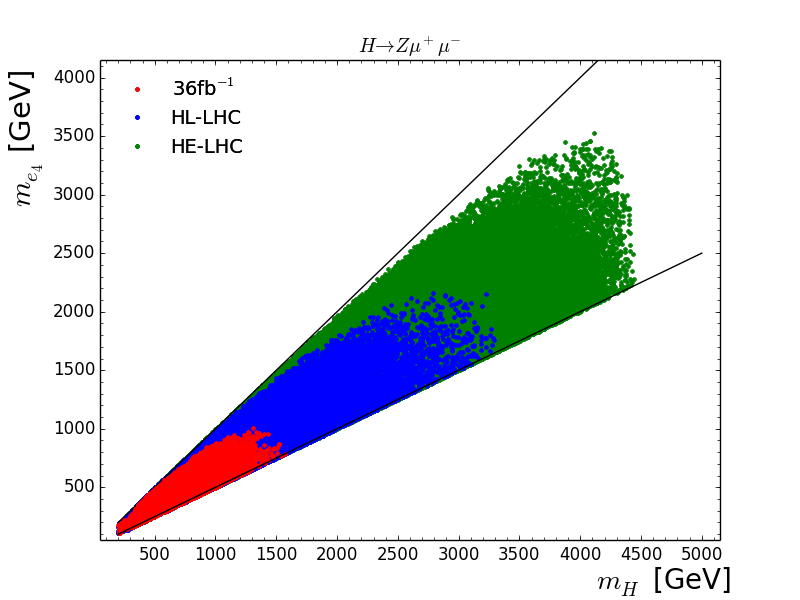
\includegraphics[width=0.49\linewidth]{\main/section7OtherSignatures/img/fig-HEHL-mH-me4-Zmumu.png}
\caption{
Experimental sensitivities for $H \to e_4^\pm \mu^\mp \to h \mu^+ \mu^-$ (left) and $H \to e_4^\pm \mu^\mp \to Z \mu^+ \mu^-$ (right) in the $[m_H,m_{e_4}]$ plane. Note that we require $m_H>m_{e_4}$ to allow the decay channel, and that we loose sensitivity for $m_H > 2 m_{e_4}$, where the $H\to e_4 e_4$ branching ratio dominates. See the caption in \fig{fig:mHtanbe} for further details. 
}
\label{fig:mHme4}
\end{figure}
%--

%Finally, let us comment on Higgs cascade decays through vectorlike quarks. The event topologies are depicted in \fig{fig:VLQtopologies}. The possible final states are $Wtb$, $Zt \bar t$, $Zb \bar b$, $h t \bar t$, and $h b \bar b$. In \fig{fig:scansigbr} we show typical production rates normalized to the cross section of a heavy SM-like Higgs boson. These final states are more challenging to study because of large QCD backgrounds but are nevertheless promising due to sizable cross sections. 
%
%%
%\begin{figure}
%\begin{center}
%%
%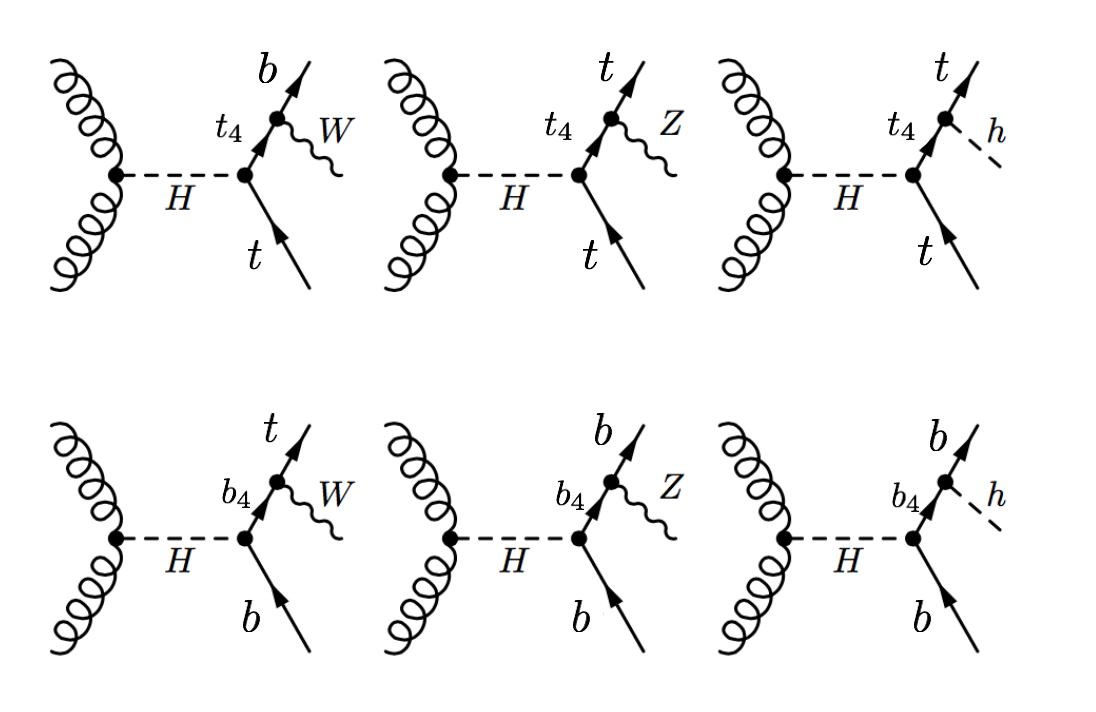
\includegraphics[width=0.7\linewidth]{\main/section7OtherSignatures/img/vlq-fig.png}
%%
%\caption{Heavy Higgs boson cascade decays through vectorlike quarks.
%\label{fig:VLQtopologies}
%}
%\end{center}
%\end{figure}
%%
%
%%--
%\begin{figure}
%\centering
%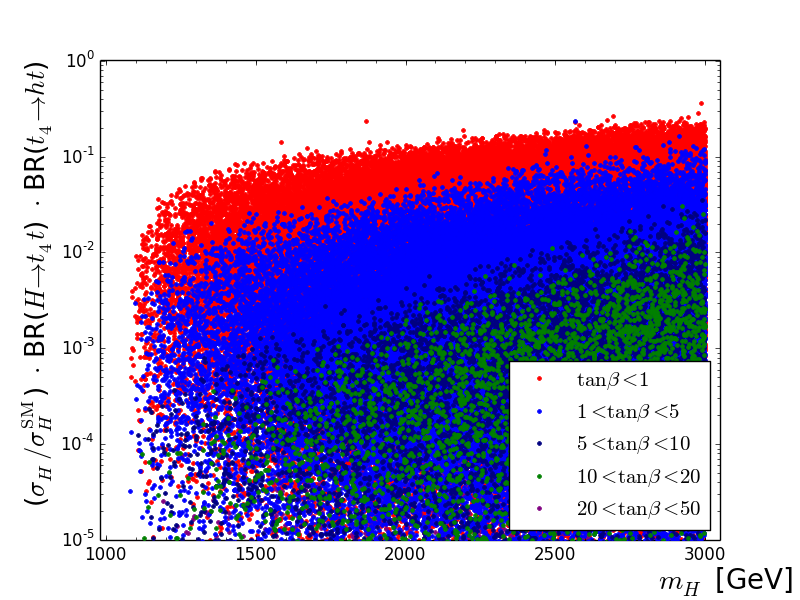
\includegraphics[width=0.49\linewidth]{\main/section7OtherSignatures/img/t1ewpt-sigBR.png}
%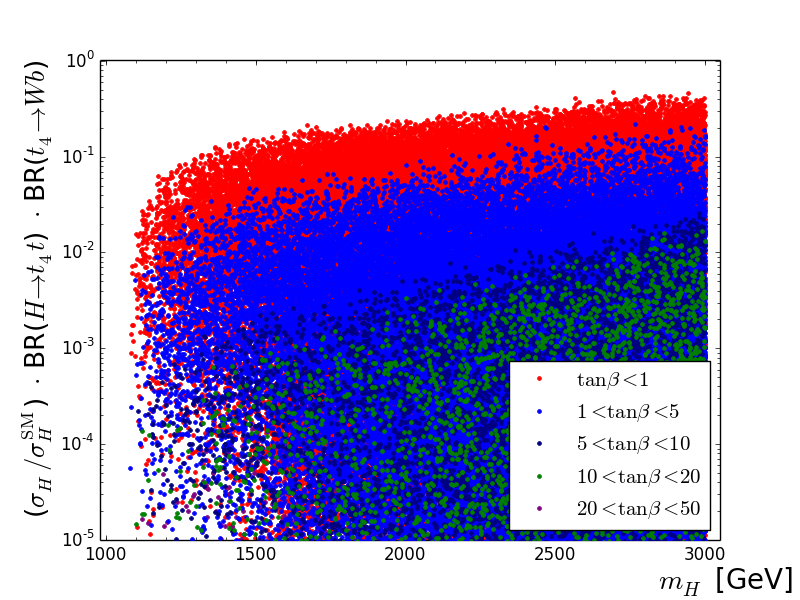
\includegraphics[width=0.49\linewidth]{\main/section7OtherSignatures/img/t1ewpt-sigBRw.png}
%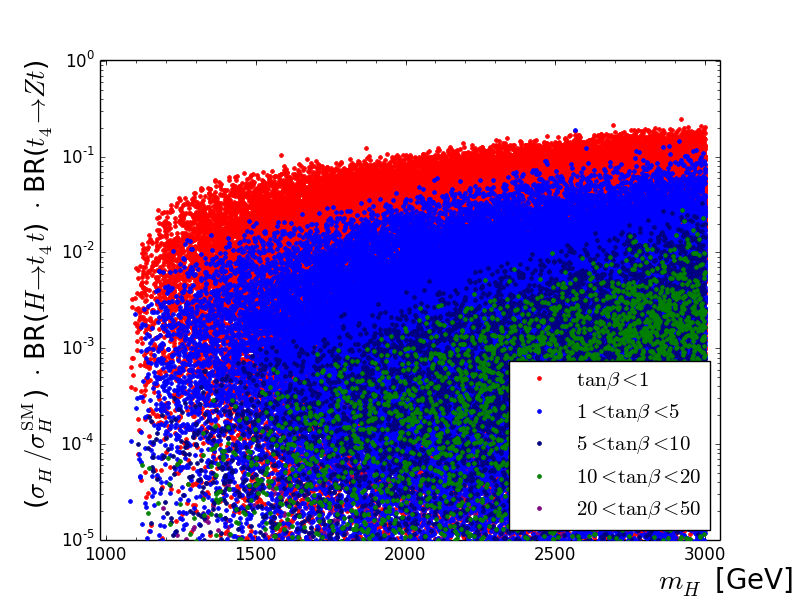
\includegraphics[width=0.49\linewidth]{\main/section7OtherSignatures/img/t1ewpt-sigBRz.png}
%\caption{
%Possible values of $(\sigma_H / \sigma_H^{\rm SM}) \times  {\rm BR}(H \to t_4 t) \times {\rm BR}(t_4 \to h t)$, $(\sigma_H / \sigma_H^{\rm SM}) \times  {\rm BR}(H \to t_4 t) \times {\rm BR}(t_4 \to w b)$, and $(\sigma_H / \sigma_H^{\rm SM}) \times  {\rm BR}(H \to t_4 t) \times {\rm BR}(t_4 \to z t)$. For $m_H \in [1.2 \; {\rm TeV},3\;{\rm TeV}]$, the cross section for SM-like heavy Higgs production varies in the ranges $[38\; {\rm fb}, 0.03\; {\rm fb}]$  and $[300 \; {\rm fb}, 1 \; {\rm fb}]$ fb at 13 and 27 TeV, respectively.
%}
%\label{fig:scansigbr}
%\end{figure}
%%--
